\begin{figure}[t]
\centering
    \begin{subfigure}{0.40\textwidth}
    \centering
    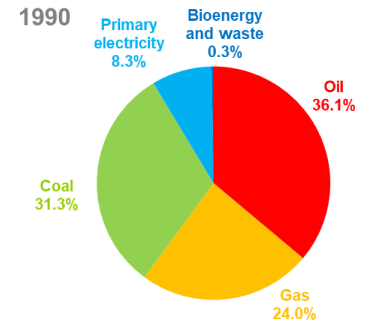
\includegraphics[height=5cm]{assets/graphs/energy-consumption_1990.png}
    \end{subfigure}
    \begin{subfigure}{0.40\textwidth}
    \centering
    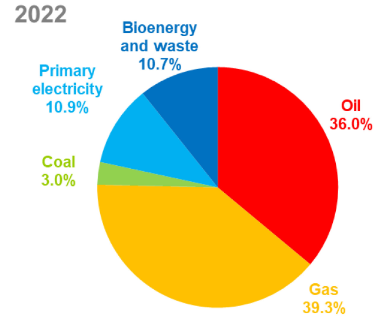
\includegraphics[height=5cm]{assets/graphs/energy-consumption_2022.png}
    \end{subfigure}
\caption{Total energy production in the United Kingdom in 1990 and 2022 \cite{departmentforenergysecurityandnetzero2023UKEnergyBrief}.}
\label{fig:fuel-consump}
\end{figure}

The growth of international populations and industry have meant that the global market for energy is higher than ever \cite{newell2019GlobalEnergyOutlook} and the reliance on fossil fuels is ubiquitous despite international efforts to quell carbon emissions \cite{unitednations2015ParisAgreementUNFCCC}. Nevertheless, with the price of green energy at its lowest historical levels \cite{internationalrenewableenergyagency2022RenewablePowerGeneration} and the threat of irreversible climate crises imminent, work must be done to adopt renewable energy sources. In Britain, the removal of coal as an energy source was successful, as shown in \fig{fig:fuel-consump}. This \emph{fuel switching} from coal to gas and oil, promoted by effective economic factors, led to a 6\% decrease in the country's overall carbon emissions despite an increase in overall energy consumption \cite{wilson2018RapidFuelSwitching}. With natural gas, methane is almost exclusively burnt and the domestic and industrial sectors account for approximately a third each (237 TWh and 206 TWh of methane, respectively) of the total methane consumption in Britain in 2023 \cite{departmentforenergysecurityandnetzero2023HistoricalGasData}.

One appropriate renewable source of energy is that of hydrogen, which is unlikely to replace the usage of fossil fuels but may be used alongside gas in applications where gas was already being burnt \cite{momirlan2005PropertiesHydrogenFuel}. Combustion of hydrogen with air is usually performed lean to avoid the NO$_x$ pollution risk under stoichiometric hydrogen-air combustion. Although lean hydrogen combustion is greener than gas or oil, different hydrogen production processes \cite{dasilvaveras2017HydrogenTrendsProduction} cause various carbon emissions \cite{nationalgrid2022HeatingOurHomes}. Hydrogen represents an attractive energy source \cite{momirlan2005PropertiesHydrogenFuel}, particularly through fuel cells \cite{momirlan2005PropertiesHydrogenFuel} and combustion \cite{lanz2001Module3Hydrogen, stepien2021ComprehensiveOverviewHydrogenFueled}. The combustion of hydrogen in particular may be used for internal combustion engines, gas turbines cookers and gas boilers \cite{momirlan2005PropertiesHydrogenFuel}. It has also been estimated that by 2040, the demand for hydrogen in the United States will have grown to 15 million tons \cite{molkov2007HydrogenSafetyResearch} and represents the growth of the \emph{hydrogen economy}.

Hydrogen presents significant safety concerns \cite{green2006HydrogenSafetyIssues} especially in its gaseous form, with an obvious example of this being the 1937 Hindenburg disaster \cite{dilisi2017HindenburgDisasterCombining}. One probable cause of this was the light H\sub{2} molecules escaping the Zeppelin and catching alight. Beyond this, lean hydrogen-air combustion is subject to two primary instabilities which pose challenges to engineering applications. The high mass diffusion of hydrogen results in significant \emph{thermodiffusive instabilities}, where the flame spontaneously wrinkles and curves, forming many small cellular structures \cite{sivashinsky1983InstabilitiesPatternFormation} and massively increasing the speed of hydrogen consumption \cite{howarth2023ThermodiffusivelyUnstableLeanPremixed}. Lean hydrogen-air combustion also has an acute sensitivity to \emph{thermoacoustic instabilities}, where perturbations in heat release from the flame couple to the acoustic modes of the combustor geometry, resulting in feedback. This can cause significant damage to combustors due to the extra mechanical work being done \cite{morgans2024ThermoacousticInstabilityCombustors}. Beyond these, the \emph{Darrieus-Landau instability} (also known as DL or hydrodynamic instability) is an intrinsic property of premixed flames which all are subject to, but pose little threat on their own to combustion applications as the resulting flames are attracted to a steady, albeit wrinkled, state \cite{matalon2018DarrieusLandauInstability}. Of particular interest are how these fuels behave in complex geometries, especially for the purposes of porous media combustion (PMC). The benefits and applications of PMC are wide-reaching: PMC enables more effective transfer of heat from the combustion reaction to combustor \cite{mujeebu2009CombustionPorousMedia}; hydrogen combustion in PMCs enable leaner combustion \cite{tseng2002EffectsHydrogenAddition}; PMC has been used on the smallest scales, including in micro thermophotovoltaic systems \cite{pan2015HydrogenOxygenPremixed}; and PMC has been used for the passive control of thermoacoustic instabilities \cite{meadows2015PorousInsertsPassive, dowd2018ThermoacousticInstabilityModel}.

Analytic studies form the foundation of instability research and provide many predictions for reduced-order flames in simple geometries, but fall short in the case of these complex geometries and non-idealised flames. The next tool in our tool belt is \emph{Direct Numerical Simulation} (DNS) \cite{orszag1970AnalyticalTheoriesTurbulence}, where the equations of motion are simulated directly using a fine discretisation to ensure all fluid phenomena is fully resolved. Usually, discretisations are performed on an unstructured mesh which is body-fitted to accurately represent the model geometry. Provided low-order discretisations aren't used a coarser discretisation length scale results in decreased computational cost, especially for three-dimensional simulations. Often the task of creating the mesh which minimises discretisation error is an expensive task within itself. This motivates a need for mesh-free methods which ditch connectivity in favour of local stencils around each node in a point cloud \cite{garg2018MeshfreeMethodsComprehensive, li2002MeshfreeParticleMethods}. The \emph{Local Anisotropic Basis Function Method} (LABFM) \cite{king2020HighOrderDifference, king2022HighOrderSimulationsIsothermal} is one such method, analogous to centred finite difference schemes where weights are gradient operators are approximated by weighted sums of the surrounding differences in function values from the central value. By increasing the stencil size used, improved accuracy can be achieved at the cost of computational cost. LABFM discretisations have been successfully used to model complex flame instability phenomena \cite{king2024MeshFreeFrameworkHighOrdera, broadley2025HighorderMeshfreeDirect}.

The hydrodynamic and thermodiffusive instabilities are intrinsic to premixed flames and as such can be studied by performing DNS in the small region around the flame, so full combustor geometry need not be modelled to get an accurate understanding of their nonlinear behaviour. In these cases the effect of acoustic feedback can be effectively undercut by imposing non-reflective boundary conditions on inflows and outflows. Using the \emph{Navier-Stokes Characteristic Boundary Conditions} (NSCBCs) developed by \cite{thompson1990TimeDependentBoundaryConditions, poinsot1992BoundaryConditionsDirect, poinsot2001TheoreticalNumericalCombustion, sutherland2003ImprovedBoundaryConditions} non-reflective boundary conditions can be imposed which allow only small reflections of acoustic waves back into the computational domain. On the other hand, thermoacoustic instabilities -- besides the recently discovered intrinsic thermoacoustic modes \cite{silva2023IntrinsicThermoacousticInstabilities} -- require spatial modelling of the very small scale chemical processes as well as the large scale combustor geometry. Temporally, they are bottlenecked by the speed of the implied acoustic waves. The motion of the flame within this combustor poses an additional challenge as some form of adaptive methods are typically required to accurately discretise the moving flame region. In practice, this makes it prohibitively expensive to perform DNS of full thermoacoustically unstable flames in, e.g. engines and so cheaper methods like Large Eddy Simulation (LES) and Reynolds-Averaged Navier-Stokes (RANS) are used, compromising accuracy in the flame region to render the large scale acoustics \cite{yang2015LargeEddySimulationPresent, domingo2023RecentDevelopmentsDNS}.

In last years report, we performed a holistic review of combustion and flame instabilities, especially as they relate to hydrogen combustion. As background, the combustion equations were introduced alongside reasoning for the model assumptions made therein. Simplifications were made to show how these equations can be simplified into something more mathematically tractable. Details of numerical methods used to perform DNS were only briefly discussed. Initial findings given into the hydrodynamic instability and how successful qualitative models like the Michelson-Sivashinsky equation \cite{sivashinsky1977NonlinearAnalysisHydrodynamic, michelson1977NonlinearAnalysisHydrodynamic} fail to quantitatively match the flame shape for a unity Lewis number flame were given. A spectral solver was developed to more accurately model the flame in the case of high heat release, but this failed to account for the surrounding non-negligible velocities transverse to the flame.

This report is split into seven chapters, six of which remain. \chap{ch:combust-model} reiterates the combustion equations under a broad combustion model (which is the one simulated later on) and defines relevant constants used throughout the report. In \chap{ch:lit-review} we do a deep-dive into the literature of two areas of interest: thermoacoustic instability phenomena and their modelling as well as computational combustion modelling. For the former we place particular emphasis on the physical mechanisms behind the primary, secondary and intrinsic thermoacoustic instabilities and how analytic and computational modelling has been used to elucidate this work. In the latter we discuss the simulation paradigms common in combustion and turbulence modelling alongside discretisation methods and boundary conditions with relation to reproducing and studying these thermoacoustic phenomena.






